\section{Analyses \& Results}
\label{sec_analyses}

\subsection{RQ1: Comparison of tagged and untagged time-series}
Our principal research question is whether listening patterns for tagged content are consistent with the expectation that tags serve as memory cues. If this were to be the case, we would expect to see an increase in a user's listening rate to musical artists after the user has tagged them, under the assumption that a tag facilitates retrieval and increases the chances of a user listening to a tagged artist. 

Unfortunately, several factors combine to make such an analysis difficult.  First and foremost, the desired counterfactual of the untagged ``version'' of a particular tagged series, which would allow a direct testing of how tagging changes listening behavior, does not, of course, exist. We thus must utilize untagged time-series in a way that allows them to approximate what a true counterfactual might look like.  In searching for such samples, a second difficulty that arises is that listening rates for tagged time-series are much greater than for untagged time-series (the average number of total listens across time-series is 16.9 when untagged and 98.9 when tagged). While suggestive of the importance of tagging, this unbalance also suggests that controls must be instilled in both sample selection and statistical analysis to account for previous listening behavior prior to tagging. Finally, the actual point in time at which tags are expected to increase listening behavior for any given user is unknown. Thus, we must formulate our analysis to account for this uncertainty.  
%to understand how it changes behavior
%as it is theoretically possible that tagging may affect listening behavior as much three months after the tag has been placed as it does in the immediately following month.

%meticulously
To alleviate issues with the non-existence of a true counterfactual, we subselect from both the tagged and untagged series using the following formal procedure. We first temporally align the tagged and untagged time-series by selecting only those tagged time-series where the tag was applied in the month of peak listening and aligning them at that peak point, and then collecting a sample of untagged time-series also aligned at the peak of listening.  Where the peak was reached in multiple months, we chose one of these at random.
%Both tagged time-series are aligned so that they are centered on the month in which they were tagged.  If multiple tags were present, we selected the tag within the month which had the most corresponding scrobbles. While there is no analogue to this point in the untagged data, we can partially resolve the issue by noting that tagging is disproportionately likely (approximately 30\%, compared to 1.1\% if the tagging month were random) to occur in a user's \emph{peak}\footnote{The month in which they listen the most times overall} listening month for a given artist. This provides a basis for aligning the tagged and untagged time-series,

%while still admitting that there is likely a reasonable span in which tagging and past listening behavior have an effect on future actions
After aligning all tagged and untagged samples in this fashion, we further limited our analysis to a 13 month period extending from 6 months prior to the peak month to 6 months after the peak. This allows us to consider a variety of ways in which listening prior to the tag may affect future behavior. Finally, we further constrain our sampling to time-series with:
\begin{itemize}
\vspace{-.5em}
\item more than 25 total listens; 
\item a peak in listening at least 6 months from the edges of our data collection period (i.e. ensuring that the period from 6 months before to 6 months after the peak does not extend beyond the limits of our data range); and
\item at least one listen 6 months prior to and after the peak (i.e. if the peak occurs in July, there should be at least one listen between January and June, and one between August and the following January).
\vspace{-.5em}
\end{itemize}

Constraining our time-series in this manner, we are left with a total of 206,140 tagged time-series.  We then randomly sampled from the 4.1M untagged time-series an equal number meeting the same three criteria.  All results below have been verified with multiple random samplings of the untagged data.

In Figure~\ref{fig:taggedVsUntagged} we plot mean playcounts, with 95\% normal confidence intervals, for each month across all tagged and untagged time-series in the subsampled data. All values are normalized by the peak, and thus values at the peak month for both the tagged and untagged lines are unity. By visually comparing the line heights before and after the peak, Figure~\ref{fig:taggedVsUntagged} shows that the mean normalized listening rate increases in the months after the peak for both tagged and untagged time-series. However, we also see a small but reliable effect wherein tagged time-series show proportionally higher mean normalized listening rates after the peak month (in which the the tag was applied) as compared to untagged time-series. This is suggestive of an increase in listening as a result of tagging.\footnote{We also observe, however, that an small but reliable lower rate of listening to tagged artist prior to peak listening. This may indicate that songs that ``catch on'' for a user more quickly (rise faster in listening from before the peak to the peak) are more likely to be tagged, a possibility to be explored further in future work.}

While Figure~\ref{fig:taggedVsUntagged} thus gives evidence that supports our hypothesis, there are two important caveats. First, as the distribution of the number of listens in any given month across all time series is heavily skewed, the mean is not fully representative of the data. Though qualitative plots of transformed variables proved to be similar, our further statistical analysis uses a log transformed version of the listening counts to account for these deviations. Second, it seems intuitively important to control for the effect of pre-peak listening behavior on post-peak listening.

 To more robustly test our hypothesis, we therefore use a regression model that incorporates previous listening behavior on post-peak behavior. Due to a lack of knowledge about the relationship between these variables and the volume of data we have, it was both unreasonable and unnecessary to assume a linear relationship between the dependent and independent variables. Because of this, we opted for a Generalized Additive Model (GAM, \cite{hastie1990generalized}) using the R package mgcv \cite{wood2001mgcv}. Our dependent variable in the regression is the logarithm of the sum of all listens in the six months after a tag has been applied, to capture the possible effect of tagging over a wide temporal window. Note, however, that qualitative results hold when testing listening for each individual month as well.
% Also of note is our choice of using the log of the dependent variable rather than a count-based regression model (e.g. a Negative Binomial regression). The model used here appeared to fit the data better based on a variety of statistical and visual goodness-of-fit tests.
Our independent variables are a binary indicator of whether or not the time-series has been tagged, as well seven continuous-valued predictors, one each for the logarithm of the sum of listens in the peak month and the six previous months.   

  \begin{figure}[t]
    \subfloat[\label{fig:taggedVsUntagged}]{%
      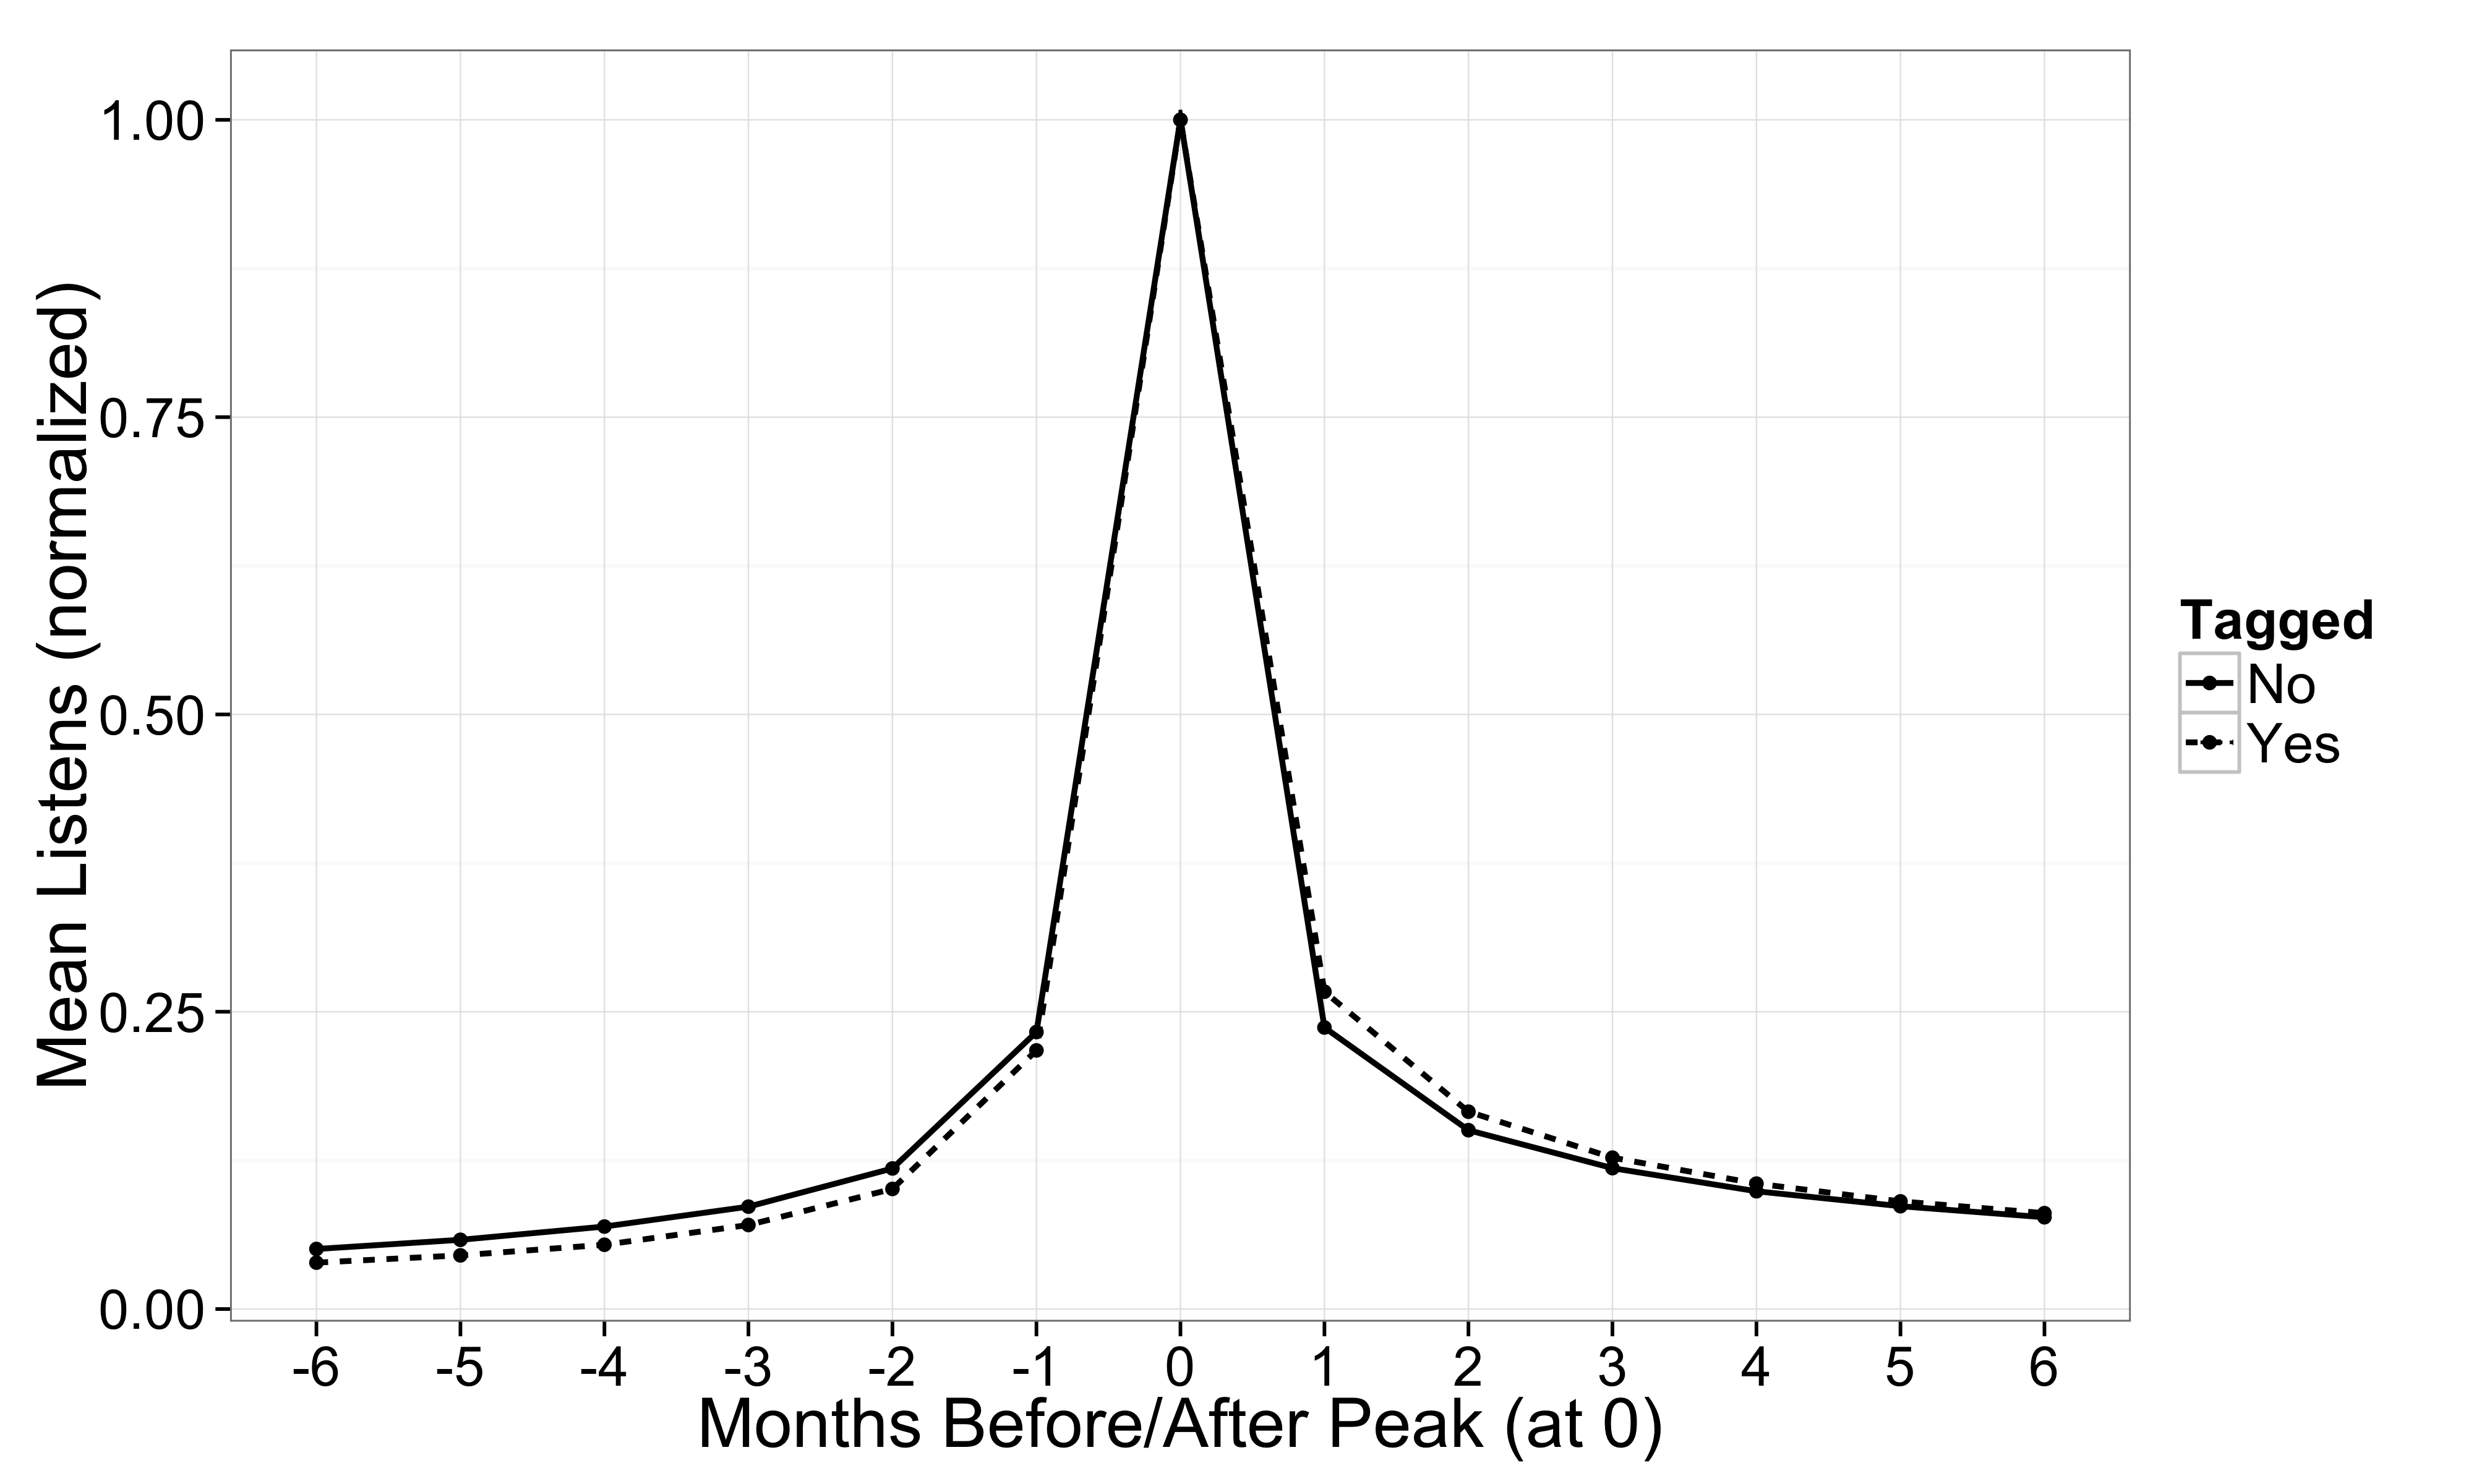
\includegraphics[width=0.45\textwidth]{taggedVUntaggedSimple.png}
    }
    \hfill
    \subfloat[\label{fig:regression}]{%
      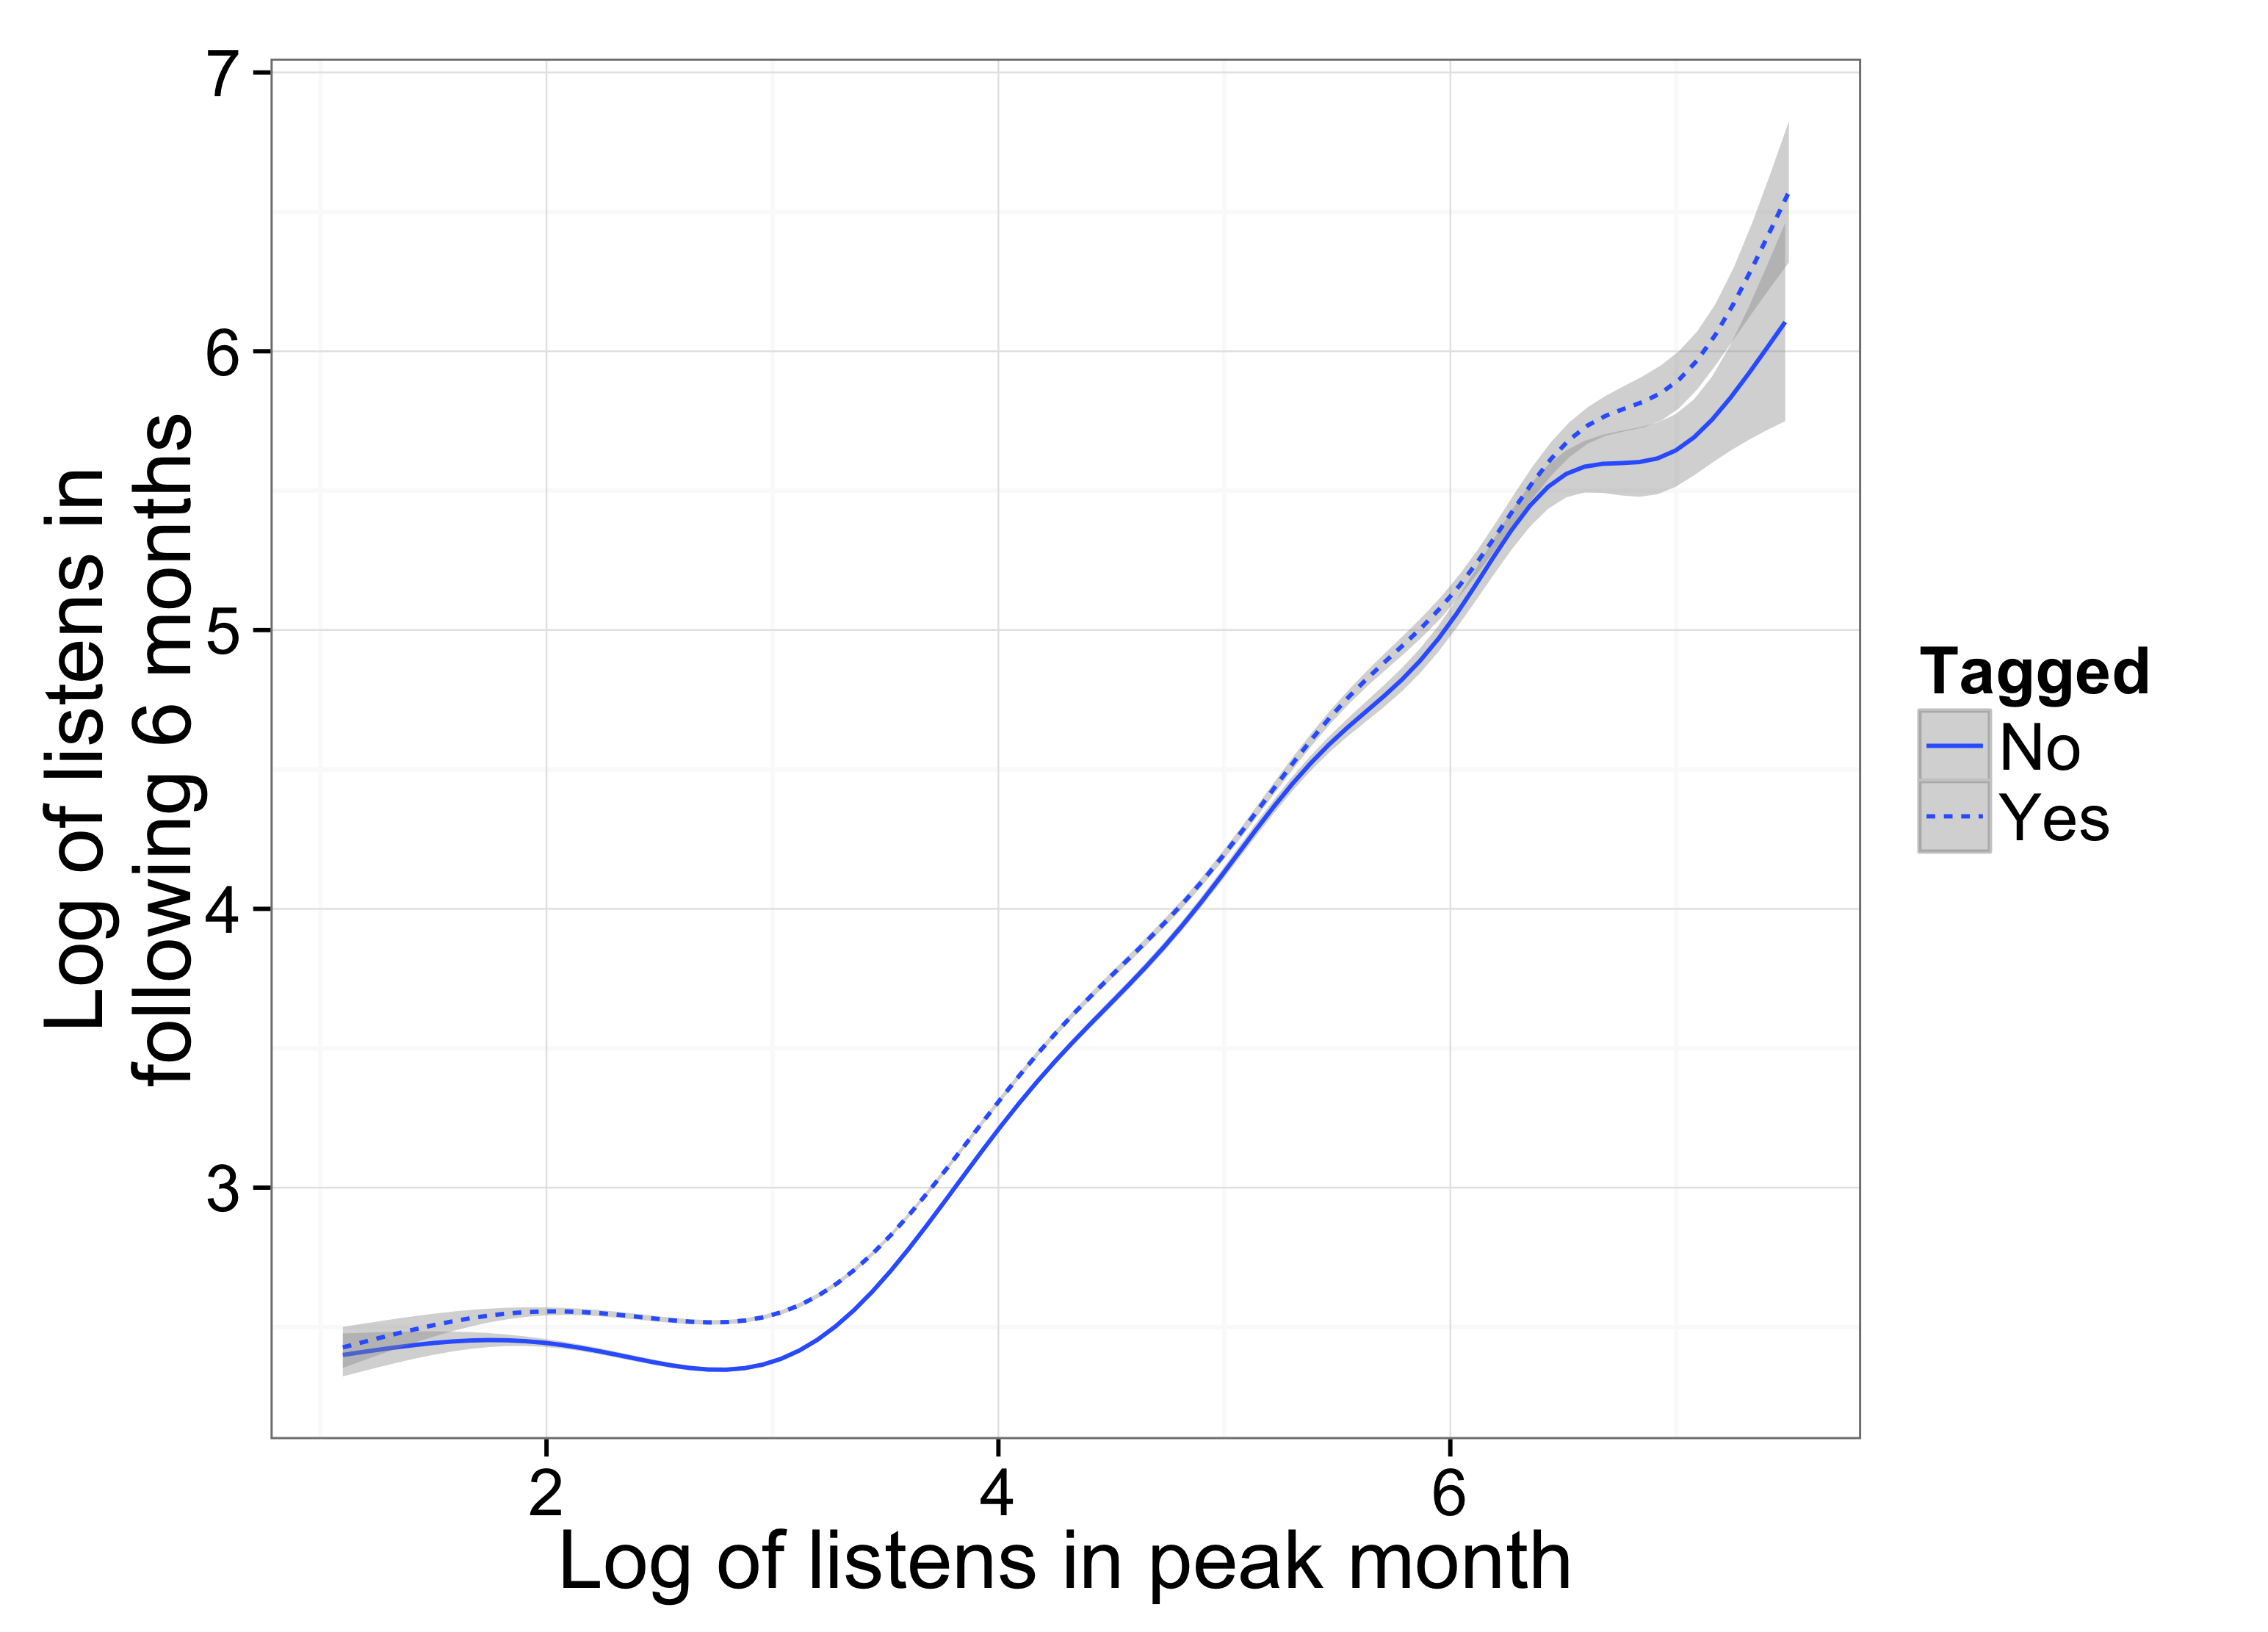
\includegraphics[width=0.45\textwidth]{taggedVUntaggedRegression.png}
    }
    \caption{Comparison of tagged and untagged listening time-series. Mean normalized playcount by month (a), and Regression results, with 95\% confidence interval (b).}
    \label{fig:regressionFigs}
    \vspace{-2em}
  \end{figure}

The regression model, which explained approximately 30\% of the variance in the data (adjusted $R^{2}$), indicated that the tagged/untagged indicator, as well as listening rate parameters (smoothed using thin-plate regression splines) for all seven previous months had a significant effect on post-peak listening behavior ($P \ll 0.0001$). As we cannot show the form of this effect for all model variables at once, Figure~\ref{fig:regression} instead displays a similar model which considers only the effect of listening in the peak month on post-peak listening. As this plot suggests and the full model confirms, we can conclude that, controlling for all previous listening behavior, a tag increases the logarithm of post-peak listens by .147 (95\% CI = [.144,.150]). This indicates that the effect of a tag is associated with around 1.15 more listens over six months, on average, than if it were not to have been applied.   

\subsection{RQ2: Tag analysis}
To examine if and how different tags are associated with increased future listening, we ran a regression analysis similar to that described above, but with two important changes. First, instead of a single tagged/untagged indicator, we included binary (present / not present) regressors for the 1,231 unique tags that had at least five occurrences in our subsample\footnote{We choose a threshold of five to ensure that data was not too sparse for the regression model but in a way that still was inclusive of infrequently occurring tags.  Again, however, we note that qualitative results hold when using both more and less restrictive thresholds.} Second, due to the data-hungry nature of the GAM and the large number of additional variables introduced by utilizing all tags as unique predictors, we chose to only use listening in the peak month (for each tag) as the independent variables. This decision limited the computational difficulties associated with estimating a model of this size and did not appear to affect model fit substantially according to tests we ran on subsamples of the data. The same data were used as in the previous analysis (untagged time series, of course, had values of zero for all possible tags).
%Four important changes were made. First, we considered only tagged time-series.  Second, instead of a single tagged/untagged indicator, we included binary (present / not present) regressors for all unique tags that had at least five occurrences in our subsample\footnote{We choose a threshold of five to ensure that data was not too sparse for the regression model but in a way that still was inclusive of infrequently occurring tags.  Again, however, we note that qualitative results hold when using both more and less restrictive thresholds.}. Third, due to the data-hungry nature of the GAM and the large number of additional variables introduced by utilizing all tags as unique predictors, we chose to only use listening in the peak month (for each tag) as the independent variables. This decision limited the computational difficulties associated with estimating a model of this size and did not appear to affect model fit substantially according to tests we ran on subsamples of the data. Finally, we eliminated the constraint that a tag must occur in the peak month of a time-series, as there is no meaningful comparison to be made with untagged data in this analysis. This allowed us to include additional tagged time-series. The dependent variable remained the log number of listens in the 6 months following tagging. If users had multiple tags for a particular artist, we again selected one tag randomly rather than include the same user artist combination twice in our analysis.

After running the model, which explains approximately 29\% of the variance in the data (adjusted $R^{2}$), 136 unique tags were statistically significant predictors at $\alpha =.001$, which we selected in order to account for the large number of comparisons against the null hypothesis being made in the regression model. While we only have sufficient evidence to make claims about these 136 tags,\footnote{Note, however, that the qualitative trends observable in the plots to follow hold regardless of the $\alpha$ threshold used.} qualitative examination of which tags are relatively strong predictors in the model proved informative.

Unsurprisinlgly, most tags tend to have a positive (albeit small) impact on future listening, as evidenced by positive regression coefficients and consistent with the small positive effect of tagging observed overall in the previous analysis. The most telling observation is that commonly-used genre tags (e.g. ``pop'', ``jazz'', and ``hip-hop'') -- which are the most common tags overall in our full dataset -- tend to be weak, positive predictors of future listening. In contrast, relatively strong predictors (both positive and negative) appear to be comparatively obscure, possibly idiosyncratic tags (e.g. ``cd collection'', ``mymusic'', ``purchased 09'').\footnote{For a full listing of the regression coefficients across all tags in the model, see \url{https://dl.dropboxusercontent.com/u/625604/papers/lorince.joseph.todd.2015.sbp.supplemental/regression_coefficients.txt}} To examine this trend quantitatively, we plot in Figure~\ref{fig:coefVsPopularity} the global tag popularity (i.e. the total number of uses of a tag in our full dataset of approximately 50 million annotations) as a function of the tag's impact on listening as indicated by its coefficient in the regression model. Similarly, we plot in Figure~\ref{fig:coefVsPopularityPeople} the unique number of users utilizing the tag, again as a function of the regression coefficients of statistically significant predictors. The value of $e^c$, where $c$ is the value of a regression coefficient, represents the number of listens we expect user's post-listening behavior to increase or decrease by if the given tag were to be applied (thus the strongest predictors lead to an increase of approximately 4.5 listens on average). Finally, in each plot, the red bands marked the upper and lower limits of a bootstrapped 95\% confidence interval on the popularity of the 1,095 remaining tags that were \emph{not} significant in the regression model. 
%, for all tags that had a statistically significant coefficient.
  \begin{figure}[t]
    \subfloat[\label{fig:coefVsPopularity}]{%
      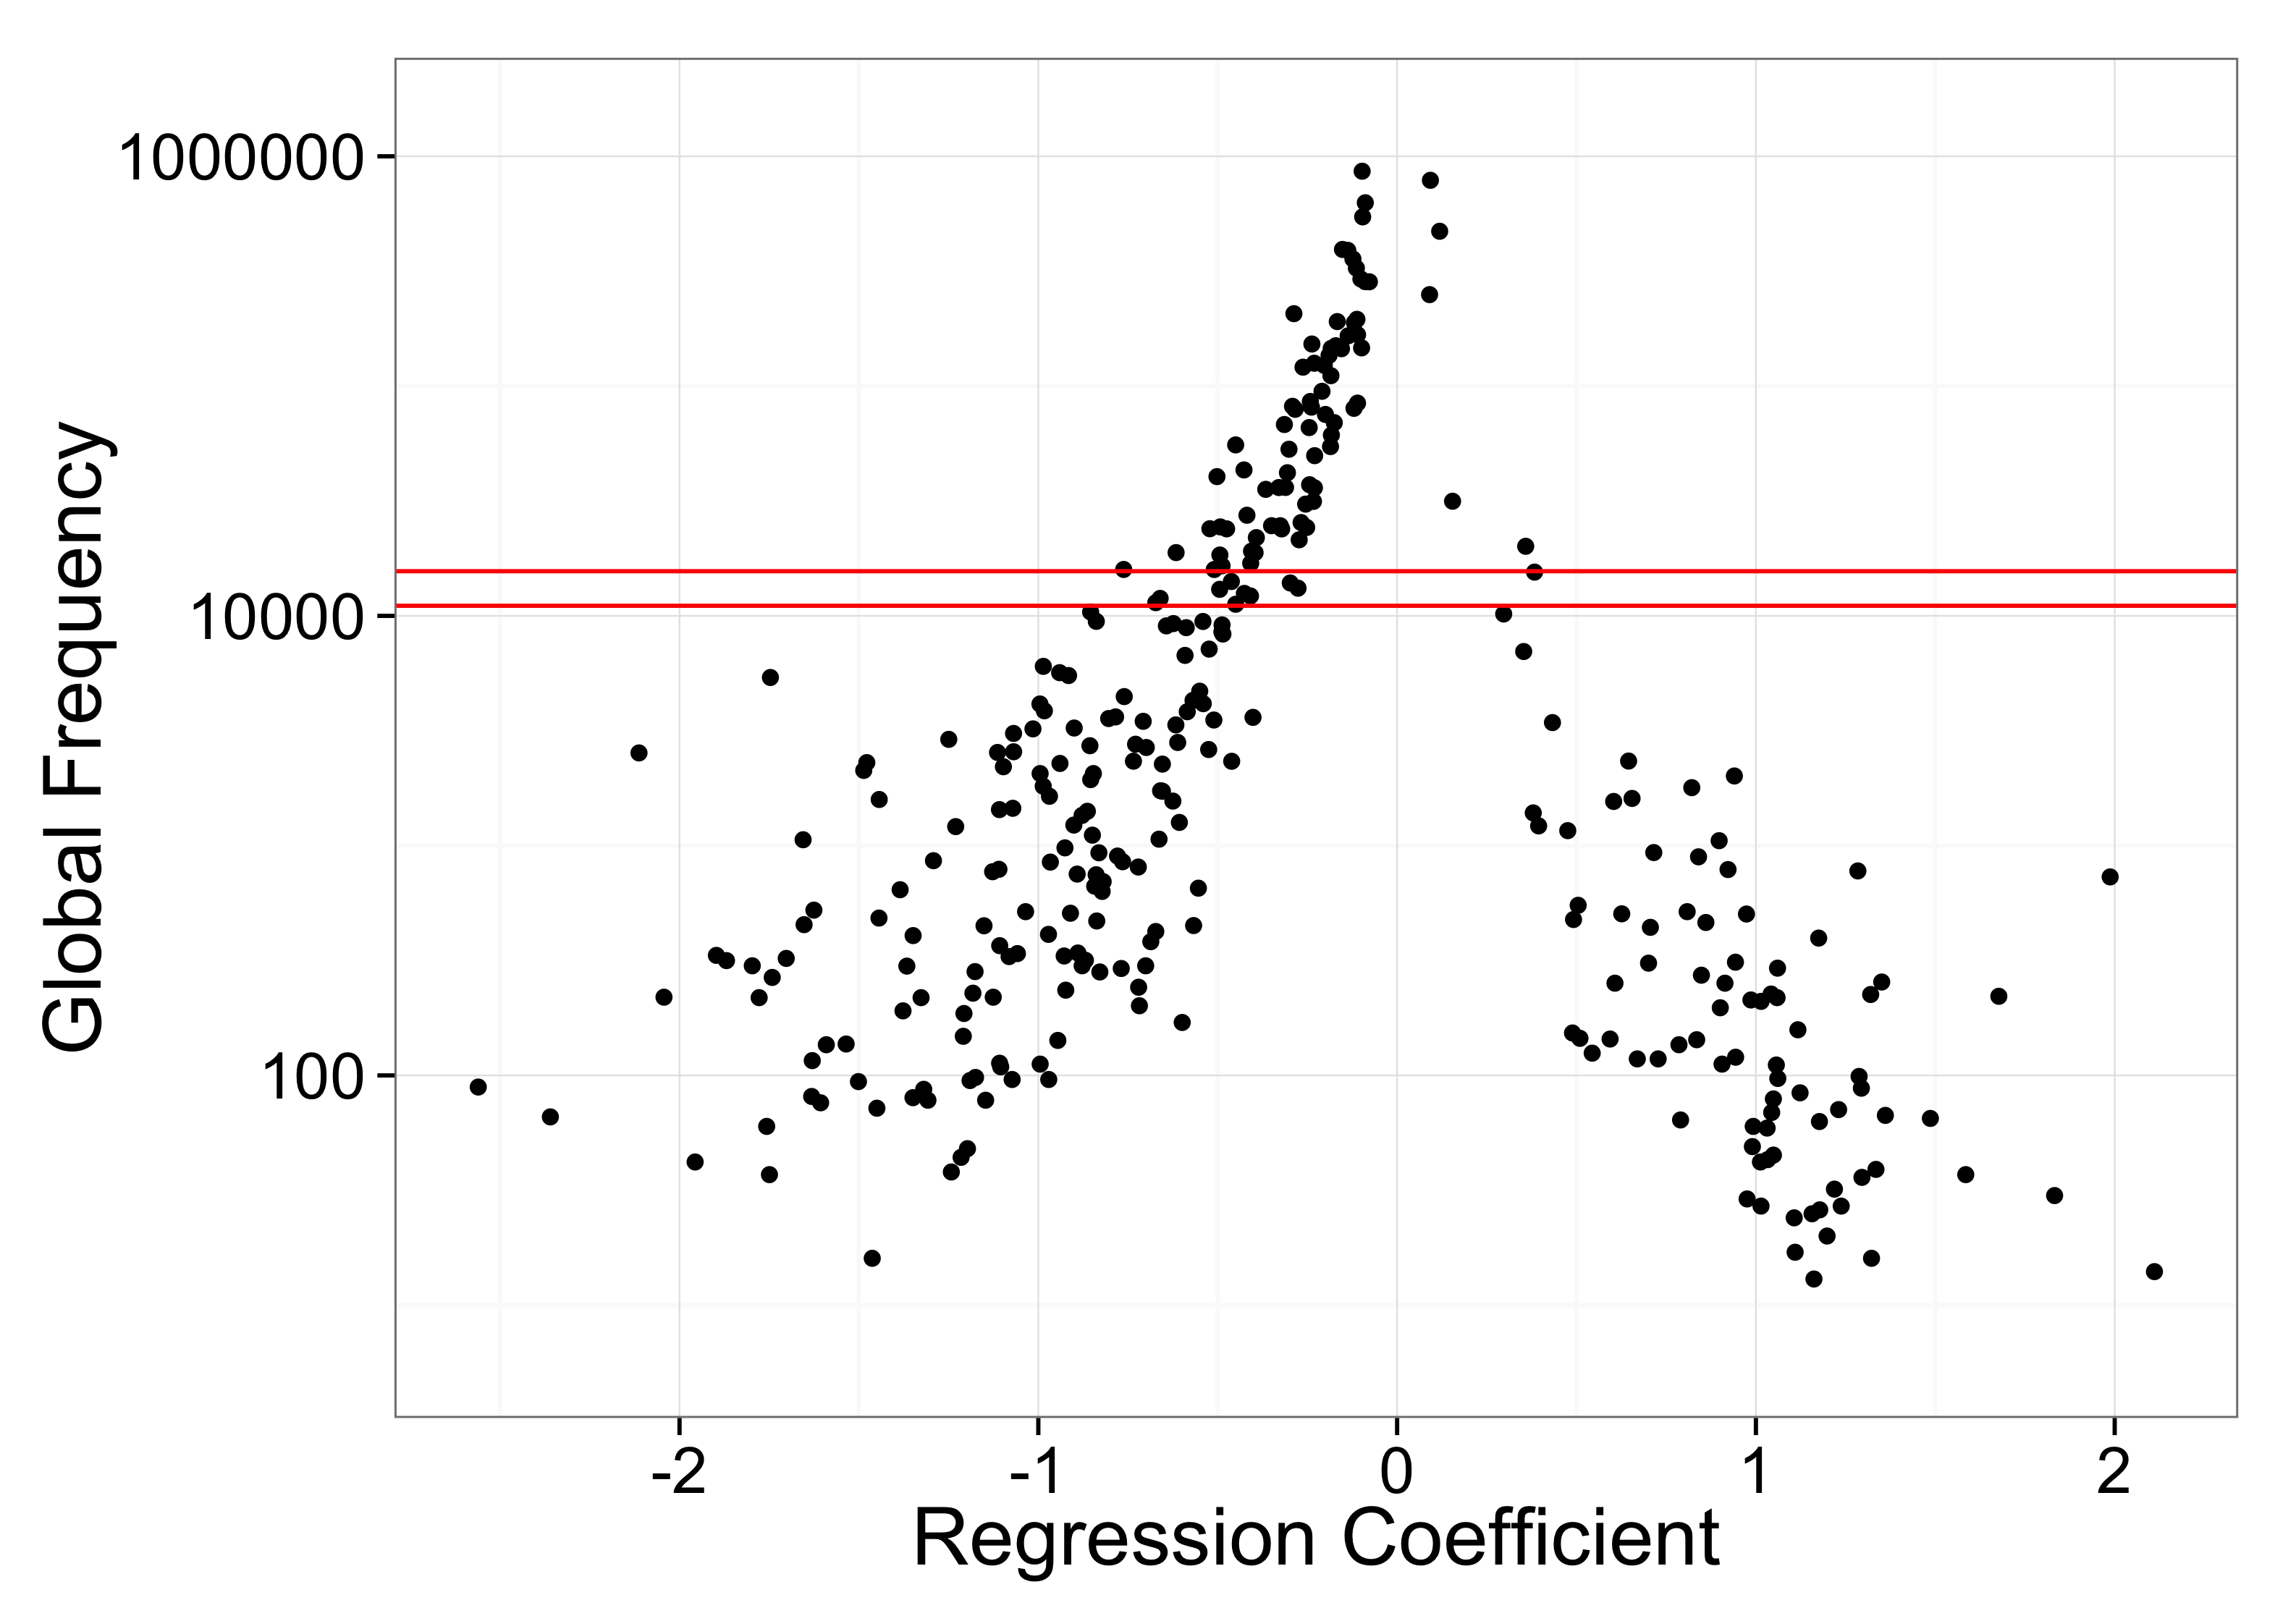
\includegraphics[width=0.45\textwidth]{tagRegressionWithMoreData.png}
    }
    \hfill
    \subfloat[\label{fig:coefVsPopularityPeople}]{%
      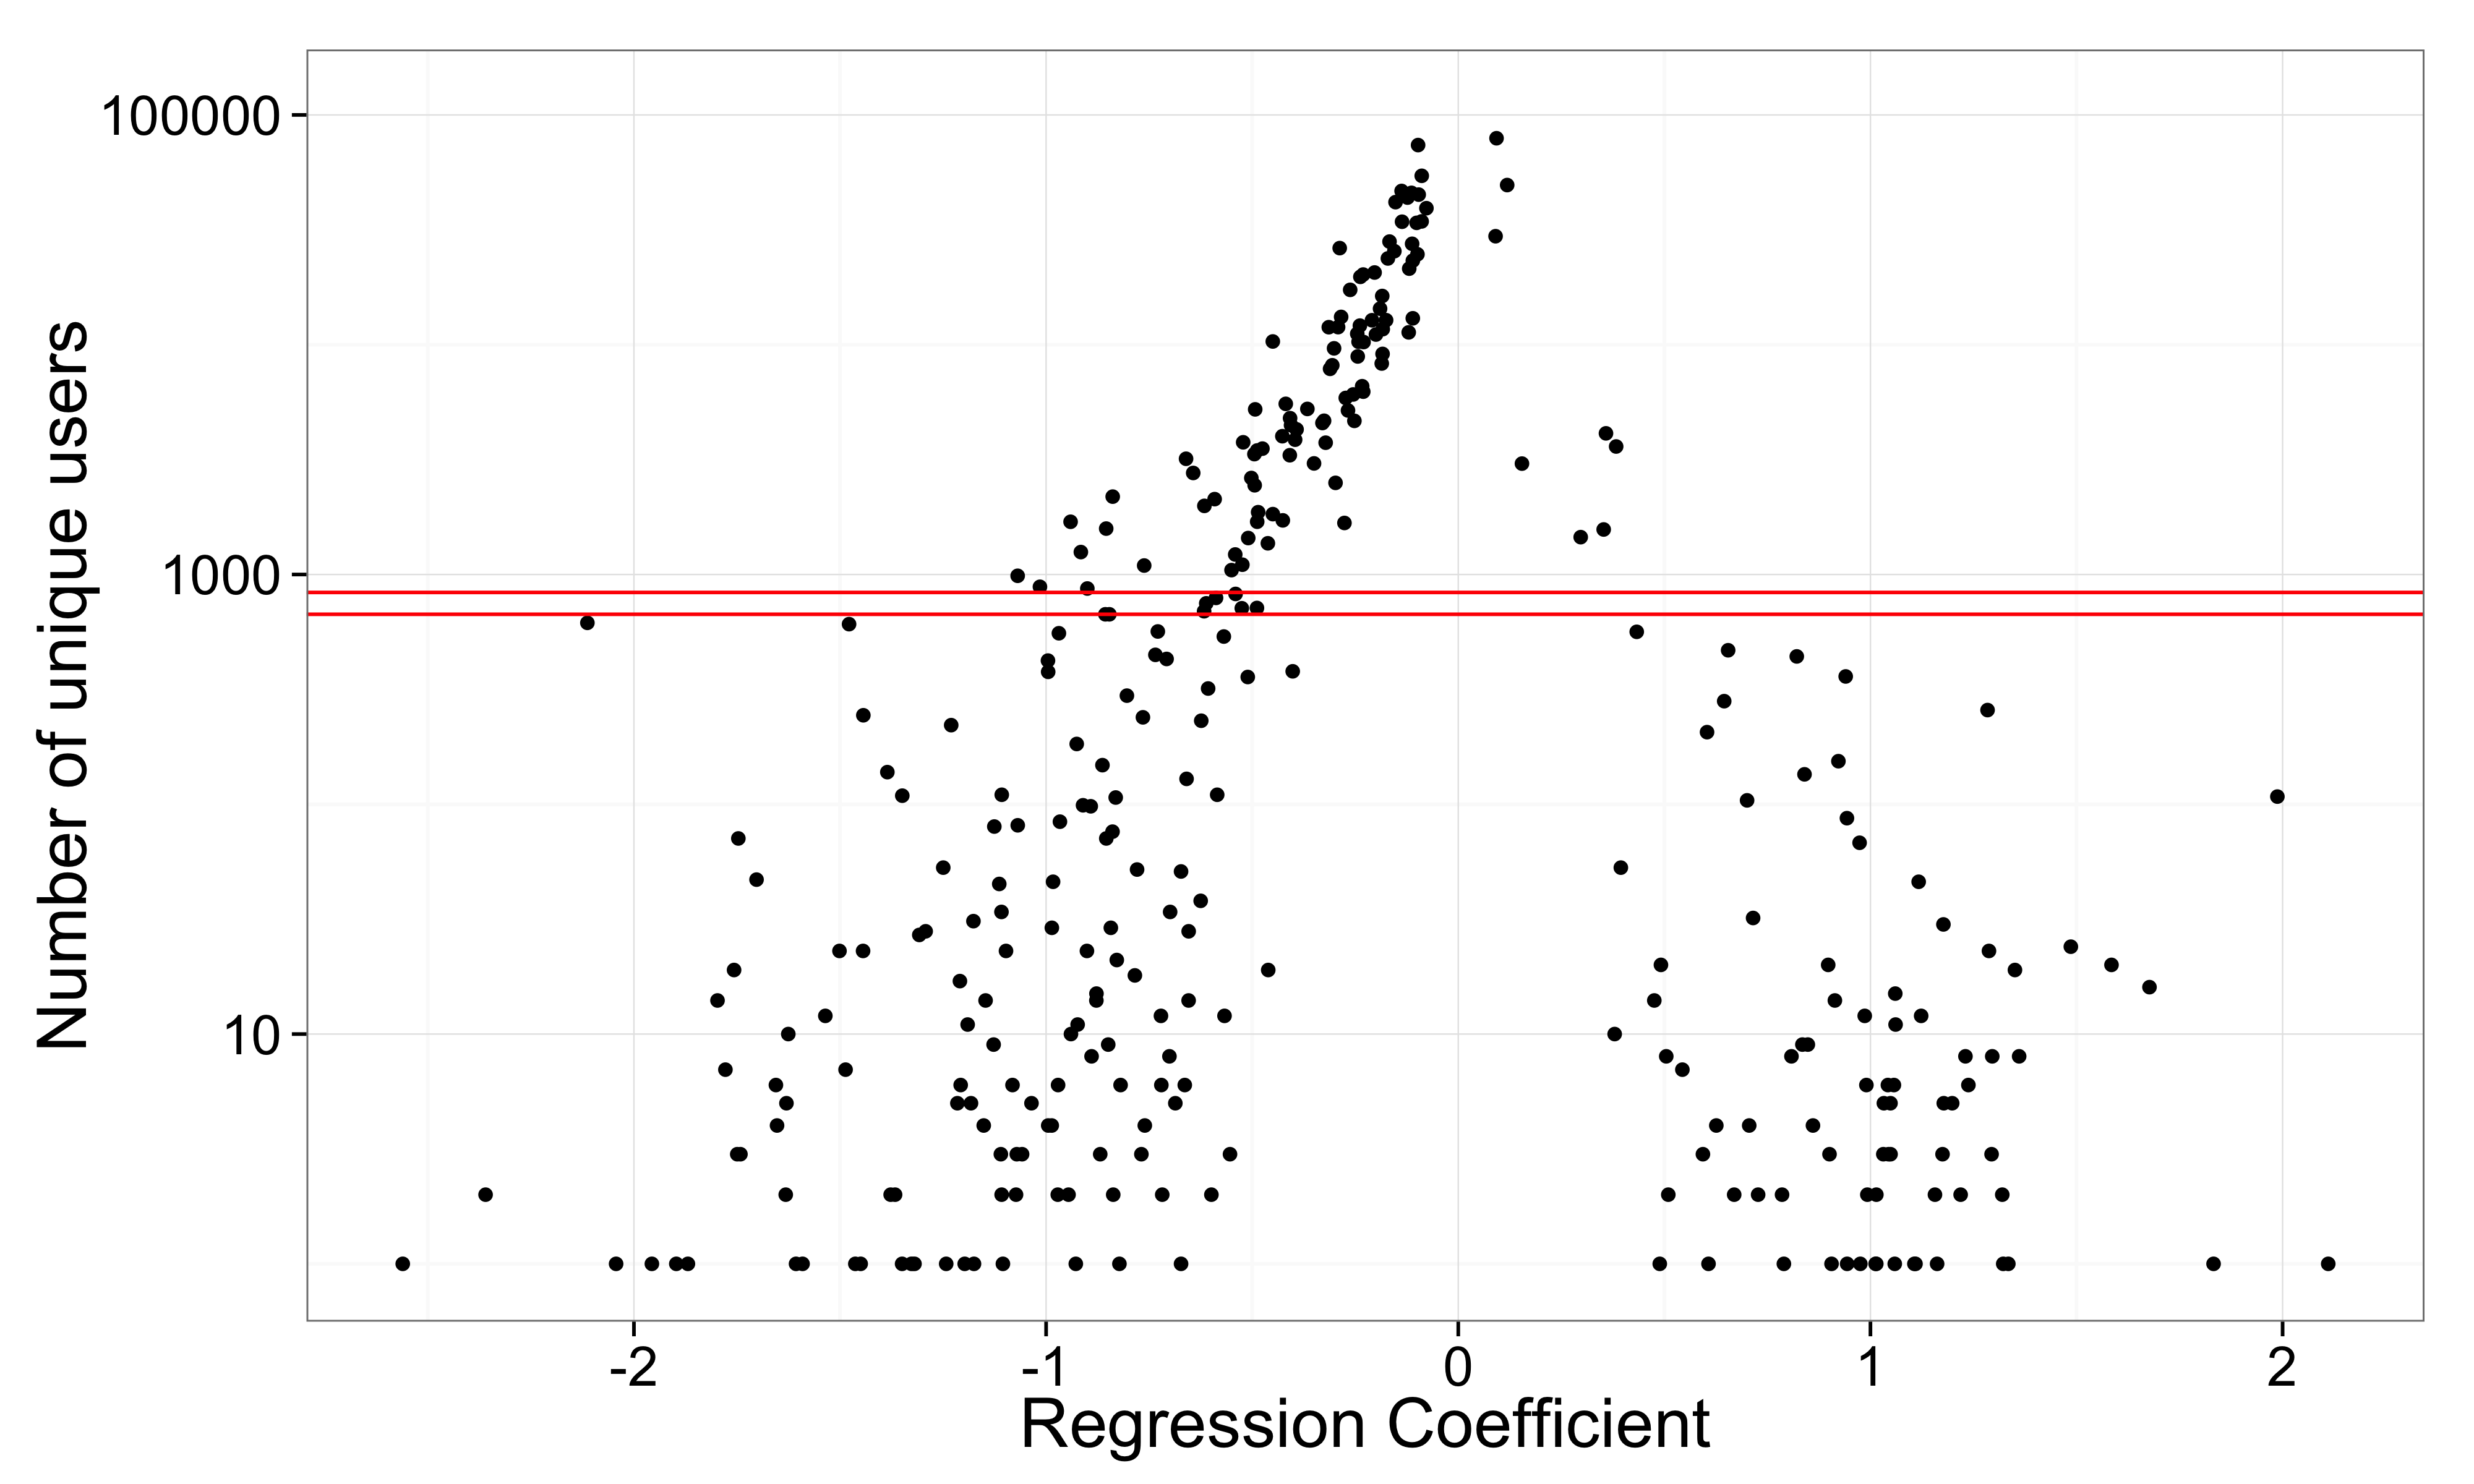
\includegraphics[width=0.45\textwidth]{tagRegressionWithMoreDataPeople.png}
    }
    \caption{In (a), the logarithm of tags' global popularity as a function of regression coefficient; in (b) the logarithm of number of unique users as a function of regression coefficient}
    \label{fig:secondPlotSet}
    \vspace{-1em}
  \end{figure}

The data suggest that the most popular tags under both metrics considered are significant, weakly positive predictors of future listening, while relatively unpopular tags tend to have relatively strong positive (and, in some cases, strong negative) impacts on listening. Tags which were not significant in the model had moderate to high popularity levels with respect to both the number of tags and the number of unique users who applied them. The high statistical reliability but small correlation coefficients for the most popular tags may be somwhat artifactual, primarily reflecting high variability in how predictive these these tags are of listening. We believe this finding is still informative, however, as it indicates that popular tags are not consistently associated with future listening.
%These data suggest that, at least for the small number of tags about which we can make statistically meaningful claims, those that are globally popular and well-known have relatively little effect on future listening, and are generally associated with small \emph{decreases} in post-taggging listening rates. The tags that seem to ``matter'' (i.e. those that are relatively strong predictors of whether or not a user will listen to an artist after tagging it) are generally much less popular.